\section{Notre outil de complétion semi-automatique}

\begin{frame}{Choix pour l'implémentation}
	\begin{columns}
		\column{0.5\textwidth}
		\textbf{Notre objectif~:}
		\begin{itemize}
			\item Reproduire un outil de complétion semi-automatique comme sur téléphone mais sur ordinateur
			\item Utilisable dans n'importe quel application
		\end{itemize}

		\column{0.5\textwidth}
		\begin{center}
			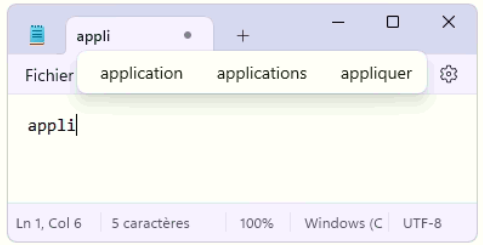
\includegraphics[width=\textwidth]{images/suggestion_windows.png}
			\uline{Outil de suggestion de mots sur Windows}
		\end{center}
	\end{columns}
	\vspace{0.5cm}
	\begin{columns}
		\column{0.5\textwidth}
		\textbf{Choix du langage~:}
		\begin{itemize}
			\item Apprendre un nouveau langage
			\item Langage de programmation moderne
			\item Conçu pour la performance
		\end{itemize}

		\column{0.5\textwidth}
		
\includegraphics[width=\textwidth]{images/rust.jpeg}
	\end{columns}
\end{frame}


\begin{frame}{Création du keylogger \& mouselogger}
	\vspace*{-0.5cm}
	\begin{columns}
		\column{0.5\textwidth}
		\begin{itemize}
			\item Détection des péréphériques
			\item Lecture des évenements
			\item Décodage avec le fichier \textbf{input-event-codes.h}
			\item Sauvegarde des évènements pour récupérer le mot tapé
		\end{itemize}
		\column{0.5\textwidth}
		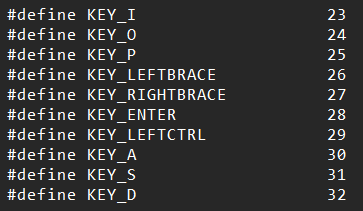
\includegraphics[width=\textwidth]{images/fichier_touche.png}
	\end{columns}
	\begin{center}
		\vspace*{-0.3cm}
		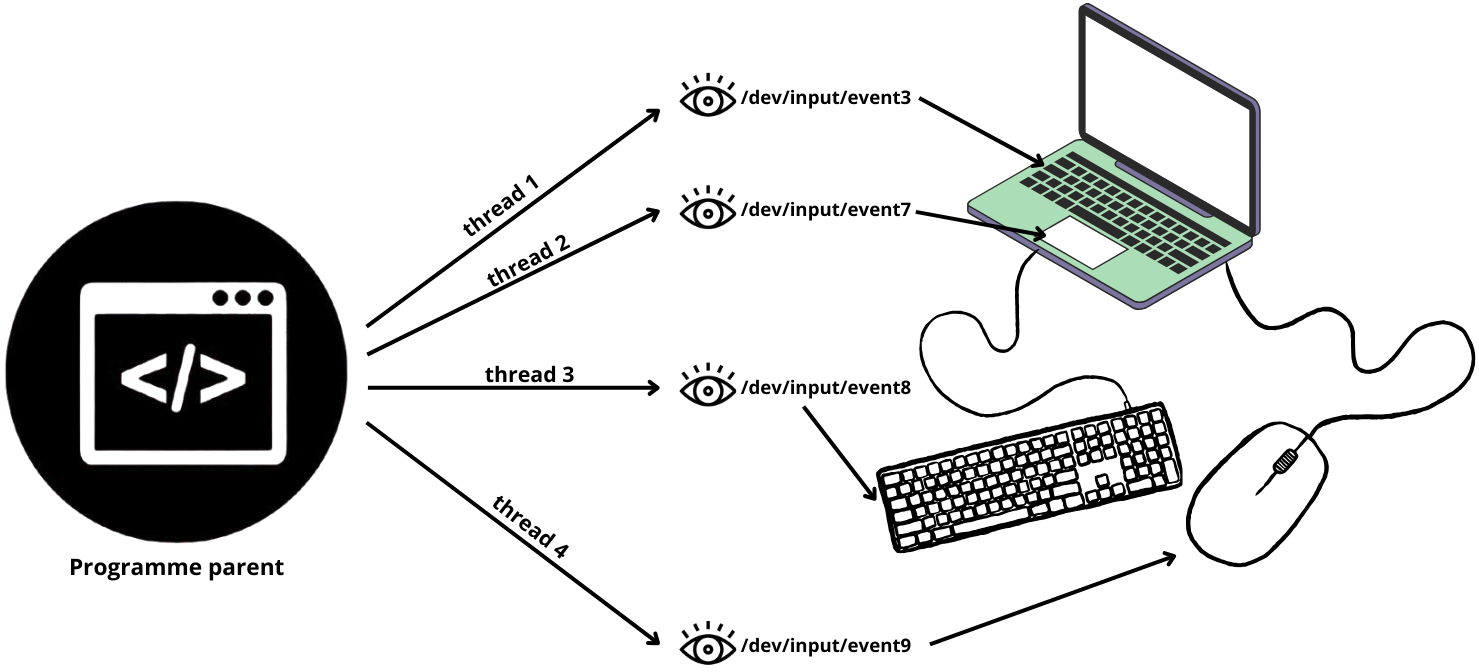
\includegraphics[width=\textwidth]{images/lecture-fichier-borderless.png}
	\end{center}

\end{frame}



\begin{frame}{Création du clavier virtuel}
	\textbf{Objectif~:} Ecrire le mot que l'utilisateur a choisi sur l'interface de l'application
	\begin{itemize}
		\item Traduction caractère → évènement clavier
		\item Envoi séquentiel des lettres du mot
		\item Suppression du mot précédent (retour arrière $n$ fois)
		\item Réécriture fluide et invisible
	\end{itemize}
\end{frame}


\begin{frame}{Algorithme de suggestion}
	Utilisation de la \textbf{distance de Levenshtein} pour la suggestion de mots

	\begin{itemize}
		\item Comparaison avec $\simeq$ 140 000 mots
		\item Sélection des mots les plus proches
	\end{itemize}

	\begin{block}{\alert{Résultats décevants}}
		→ Suggestions peu pertinentes\\
		→ Nécessité d’ajouter des critères complémentaires
	\end{block}

	\textbf{Solutions apportées~:}
	\begin{itemize}
		\item Analyse des \textbf{préfixes}
		\item Pondération selon la \textbf{fréquence d'utilisation}
	\end{itemize}
\end{frame}

\begin{frame}{Algorithme de suggestion}
	\vspace*{-0.75cm}
	\begin{center}

		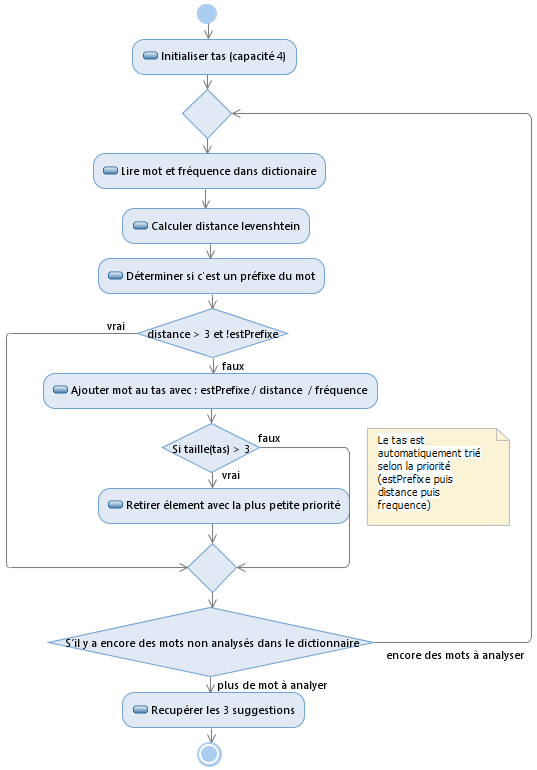
\includegraphics[height=0.98\textheight]{images/uml_diapo.png}
	\end{center}

\end{frame}




\begin{frame}{L'interface graphique}
	\begin{columns}
		\column{0.45\textwidth}
		\begin{itemize}
			\item Initialement, interface prévue en \textbf{Rust avec GTK}
			\item Problème : impossible de garder la fenêtre au premier plan constamment
			\item Solution : interface réalisée en \textbf{Python avec Tkinter}
			\item Communication entre Rust et Python via leur \textbf{entrée standard}
		\end{itemize}

		\column{0.50\textwidth}
		\centering
		\textbf{Interface finale :} \\
		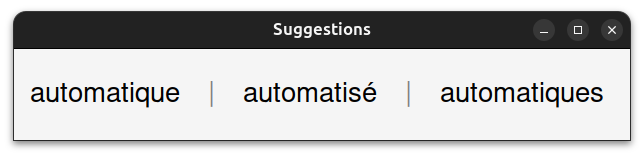
\includegraphics[width=\textwidth]{images/demo_interface.png}
	\end{columns}
\end{frame}


\begin{frame}{Installeur de l'application}
	\begin{itemize}
		\item Création d'un installeur pour l'application
		\item Utilisation d'un \textbf{Makefile}
		\item Pour
		      \begin{itemize}
			      \item Compiler le code
			      \item Attribuer les droits nécessaire
			      \item Créer le fichier \textbf{.desktop}
			      \item Déplacer le binaire
		      \end{itemize}
	\end{itemize}
	\begin{center}
		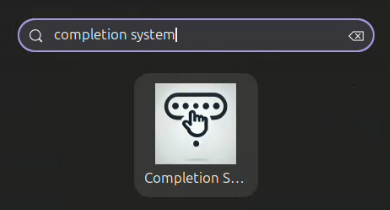
\includegraphics[width=0.5\textwidth]{images/application.png}
	\end{center}

\end{frame}

\section{Démonstration}% montrer la video
